In the previous sections we discussed how neural networks are built up. Now we will give an example of how they can be trained and used to perform specific tasks. Here, the term training refers to the search for a set of parameters $\theta$ that make a neural network with a fixed architecture behave in a desired way. Specifically, we will look at how they can be trained on data sets in a process referred to as \textbf{supervised learning}. In supervised learning, the desired behavior of a network is defined by a dataset consisting of input and output values \cite{SupervisedLearningOverview}. The network should behave in such a way that it produces the desired outputs when fed the corresponding inputs. Training consists of defining a measure of performance of the network, called the loss function, and then using mathematical iterative methods for minimizing the loss.

\subsection{Datasets}\label{sec:Datasets}
First, we need to assume that we have a given dataset containing input-output pairs that represent the task we want the neural network to perform. The neural network is supposed to learn which output is supposed to be generated from which input by evaluating the given inputs and desired outputs. We will call those desired outputs "\textbf{targets}" to distinct them from the actual outputs of the neural network. A good example of this would be the MNIST database, which was first used in 1994 in \cite{firstMNISTpaper} and has since become a popular entry-level classification task for machine learning. Examples of input data for this database are shown in \cref{fig:MNIST_examples}. 
\img{text/MachineLearningBasics/plots/mnist_plot.pdf}{14cm}{Displayed in this figure are 4 examples of input values of the MNIST dataset. This dataset represents handwritten digits from 0 to 9. Each input value consists of a 28 by 28 grid of grayscaled pixel values.}{fig:MNIST_examples}
This dataset consists of various handwritten digits from 0 to 9 represented by a 28 by 28 grid of grayscale pixel values. The values of the pixels in these grids act as the 784 input values for the neural network. The targets and the output of the neural network should be of the same shape. For example one might use a scalar output of the neural network that should be equal to the value of the digit drawn in the input pixel grid. In this case the targets are scalar values from 0 to 9 corresponding to their input pictures. Another way would be to use 10 output values together with the previously mentioned softmax function (see \cref{sec:NeuralNetworks}) to make the outputs interpretable as probabilities of each prediction \cite{gao2018properties}. We would then change our targets to vectors with 10 elements, where the entry corresponding to the handwritten digit in the input picture would be 1, every other value would be 0. For example, in this case, an image depicting the number 3 would correspond to a target of $(0,0,0,1,0,0,0,0,0,0)$.\\
We will denote the data sets as mathematical sets of input-target pairs $\{(\mathbf{x}_i, \mathbf{y}_i)\}_{i=1}^N$, where $\mathbf{x}_i$ are the input values and $\mathbf{y}_i$ are the targets. Here, we referred to the total number of training samples as $N$. The mathematical dimension of $\mathbf{x}_i$ and $\mathbf{y}_i$ can vary and are dependent on the network architecture, but we will assume that they are vectors of the real numbers $\mathbf{x}_i \in \mathbb{R}^a$ $\mathbf{y}_i \in \mathbb{R}^b$. Due to this property we also sometimes refer to them as "points". If our inputs values are organized in a different manner, for example the MNIST data being matrices of $\mathbb{R}^{28\times28}$, we can rearrange these numbers into a vector of $\mathbb{R}^{784}$ in any way we want, as long as every input is rearranged in the same manner.\\
Going further, we will denote an output of the neural network for an input $\mathbf{x}_i$ by $f_\theta(\mathbf{x}_i)$. This means that we mathematically describe the entire neural network as a function
\begin{equation}
	f: \mathbb{R}^a \times \mathbb{R}^p \rightarrow \mathbb{R}^b
\end{equation}
with $p$ being the amount of parameters in the network.

\subsection{Loss function}
Thus far, we have defined what a neural network is and how the input data we want to train on is structured. In order to train our networks to learn the underlying function of our dataset, we now need to introduce a way to measure how well our network is performing. Once we can evaluate the performance of our network, we can then introduce ways to optimize that performance.\\
This measure of the performance of a neural network is called the "\textbf{loss function}" $\mathscr{L}$. It is also sometimes referred to as the cost function in literature \cite{NGD}. Within this work, we will only consider loss functions of the form 
\begin{equation}
	\mathscr{L}\left( \{(f_\theta(\mathbf{x}_i), \mathbf{y}_i)\}_{i=1}^{N} \right) = \frac{1}{N} \sum_{i=1}^{N} \ell\left(f_\theta(\mathbf{x}_i),\mathbf{y}_i\right).
	\label{eq:Loss_longform_withFunctiondependency}
\end{equation}
Let's call $\ell$ the subloss of the system. As a reminder, $\theta$ is a set containing the parameters of the neural network, $f_\theta$ is its output function. Sometimes it's more convenient to explicitly denote the dependency on theta, which would make the loss function
\begin{equation}\label{eq:Loss_longform}
	\mathscr{L}\left( \{(\mathbf{x}_i, \mathbf{y}_i)\}_{i=1}^{N}, \theta \right) = \frac{1}{N} \sum_{i=1}^{N} \ell_\theta\left(\mathbf{x}_i,\mathbf{y}_i\right).
\end{equation}
How exactly the loss function should be defined cannot be generally stated. In any case, the value of the loss function should generally be smaller the closer the output of the neural network is to the corresponding targets.\\
In most of our cases we use loss functions with 
\begin{equation}\label{eq:DistanceLoss}
	\ell_\theta \left( \mathbf{x}_i,\mathbf{y}_i\right) = 
	d\left(f_\theta(\mathbf{x}_i), \mathbf{y}_i\right),
\end{equation}
where $d$ represents the distance between the output vector of the neural network and the target vector according to different metrics. One very would be 
\begin{equation}
	\mathscr{L}\left( \{(\mathbf{x}_i, \mathbf{y}_i)\}_{i=1}^{N}, \theta \right) = \frac{1}{N} \sum_{i=1}^{N} \sum_{j=1}^{N} \left(f_\theta(\mathbf{x}_i)_j - y_{i,j}\right)^2,
\end{equation}
with $f_\theta(\mathbf{x}_i)_j$ and $y_{i,j}$ being the $j$-th component of the network output and target vectors. Further examples and loss functions of different forms can be found in \cite{LossExamplePaper}.

\subsection{Optimization}\label{sec:NetworkOptimization}
To quickly recap, we have now defined what a neural network is and that we want a fixed network architecture during training, for which the parameters can vary to optimize the performance. We also assume that we have a data set that we want our network to learn the structure of, and a loss function that measures how well the current setup of our network is performing. We will now talk about how we can change the parameters to optimize performance.\\
This is achieved by minimizing the value of the loss function. The simplest and most common algorithm to do this with is \textbf{Gradient Descent} (GD). Here, the rule for updating the parameters looks like \cite{GradientDescentOverview}
\begin{equation}\label{eq:GD}
	\theta' = \theta - \eta \nabla_\theta \mathscr{L}\left[ \{(\mathbf{x}_i, \mathbf{y}_i)\}_{i=1}^{N}, \theta \right],
\end{equation}
where $\eta$ is a parameter of training called the "learning rate", which is a scalar value for GD but could also vary through training and even be a matrix for more advanced optimization methods \cite{ThePrinciplesOfDeepLearningTheory}.\\
The idea behind GD is that the gradient with respect to $\theta$ points in the estimated direction of the steepest ascent of the loss when the parameters are varied. If we subtract this gradient from the parameters we update the loss in the opposite direction, which is the estimated direction of steepest descent. To visualize this, let's examine a single parameter $\theta_1$. The update rule for this single parameter can be obtained from writing out the previous \cref{eq:GD} in its full vectorial component form and then picking out the line of $\theta_1$. It reads
\begin{equation}
	\theta_1' = \theta_1 - \eta \pAbl{}{\theta_1} \mathscr{L}\left[ \{(\mathbf{x}_i, \mathbf{y}_i)\}_{i=1}^{N}, \theta \right].
\end{equation}
To explain the concept of this algorithm more visually let's take a look at \cref{fig:gd_explanation_plot}. 
\begin{figure}
	\centering
	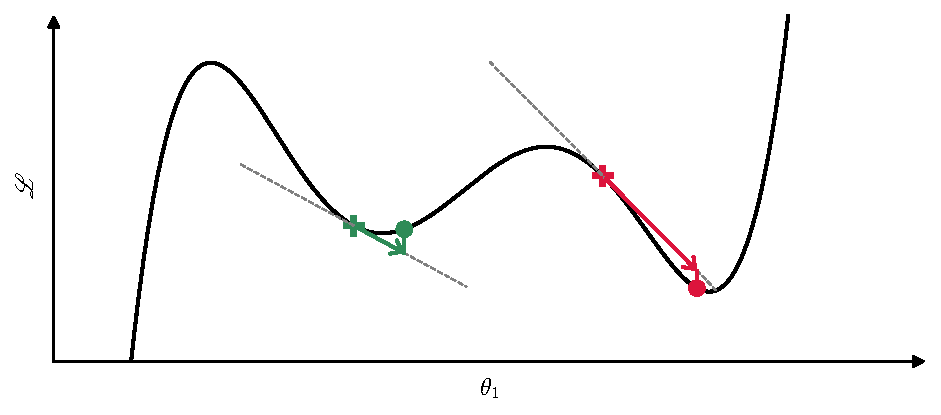
\includegraphics[width = \textwidth]{text/MachineLearningBasics/plots/sgd_plot.pdf}
	\caption{Visual explanation of the Gradient Descent algorithm. The dot markers show where a parameter that starts at the cross marker might end up if the algorithm is applied.}
	\label{fig:gd_explanation_plot}
\end{figure}
The cross markings symbolize the position of parameter $\theta_1$ before the update step. The algorithm then calculates the derivative of the loss $\pAbl{}{\theta_1} \mathscr{L}$, which geometrically is the slope of the tangent. To update the parameter, the slope is multiplied with $-1$ times the learning rate $\eta$ and added to $\theta_1$, which is represented by the arrows. The length of these arrows depicts the resulting change in $\theta_1$. One can see that the red arrow on the right covers more distance in the direction of $\theta_1$ than the green one on the left, which is a result of the corresponding slope being steeper. The circle markers then mark the updated parameter value $\theta'_1$.\\
This process of updating the parameters is repeated several times. One update is called an update step. When using batches of the dataset for parameter updates, an epoch refers to a period of training after which the algorithm calculated gradients on each input-output data pair. The number of update steps in an epoch depends on the batch size.\\ 
This visual example already illustrates some of the drawbacks of the GD algorithm: Starting training with the green parameter will yield a higher final loss than starting with the red parameter. Also going further to the left would make the loss function smaller than both of these local minima. GD just tends to find the closest local minimum instead of a global one \cite{SGDLocalMinima}. Another drawback results from the step size being finitely big, which makes the green parameter hop over the local minimum. Both of these problems can't be solved by simply optimizing the learning rate $\eta$ in general.

\subsection{Other optimizers}
The standard GD calculates the gradient for parameter updates from the whole data set according to \cref{eq:GD}. It can be sufficient or even beneficial to compute the loss gradient and update the parameters for a subset of the whole data set \cite{SGDLocalMinima}, which is usually called mini-batching. The extreme end of this would be to calculate the gradient and update the parameters for one data point each, which is then called \textbf{stochastic Gradient Descent}.
GD and its variations are very simple and fast to compute algorithms, but they generally only converge to local minima and can quite easily hop over them. That's why other algorithms have been developed, aiming to solve or mitigate some of the problems of GD. In all applications of GD to train a model in this thesis, the so-called ADAM optimizer was used. The intricacies of this optimization method are beyond the scope of this work. We refer the interested reader to \cite{adamPaper}, where the details of this algorithm are discussed. %Another optimization algorithm that can be used to overcome some of the problems of GD is the Natural Gradient Descent \cite{NaturalGradientpaper}.


